\subsection{CU9 Solicitar Refacción}
Al entrar a esta parte del sistema, se despliega esta pantalla. Es un formulario de registro para la solicitud de alguna pieza en especifico. Solicitará un identificador (en este caso manejamos un Número de Solicitud), la Fecha en que se solicita y una Descripción donde se podrá agregar alguna otra información como el nombre o modelo. 
\\
Un vez llenado el formulario el usuario podrá pulsar el botón de 'Solicitar' para registrar esto en la base de datos. En caso de que el usuario desee salir de esta pantalla, simplemente deberá pulsar el botón 'Cancelar'.
\begin{figure}[!h]
	\centering
	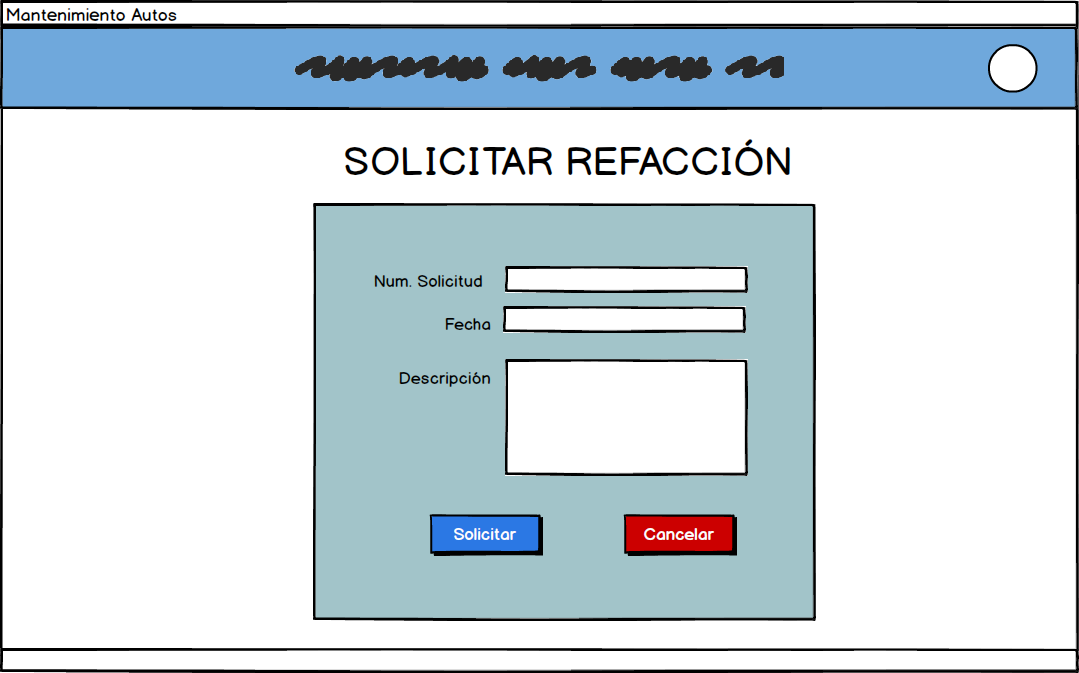
\includegraphics[width=1\textwidth]{./diseno/vescenarios/imagenes/solicitarRefaccion}
	\caption{Pantalla Solicitar Refacción - Vista de Escenarios}
	\label{fig:Pantalla Solicitar Refaccion - Vista de Escenarios}
\end{figure}
En caso de que el usuario ingrese de manera incorrecta alguno de los campos, el sistema mostrará un 'mensaje de alerta' (figura \ref{fig:Alerta5 - Vista de Escenarios}) informado del error que ha cometido. 
\begin{figure}[!h]
	\centering
	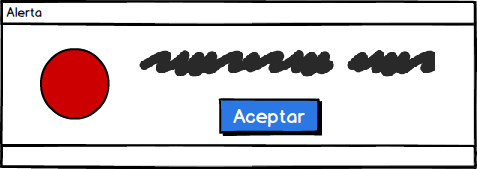
\includegraphics[width=0.4\textwidth]{./diseno/vescenarios/imagenes/alerta}
	\caption{Alerta Confirmación de Registro - Vista de Escenarios}
	\label{fig:Alerta5 - Vista de Escenarios}
\end{figure}